\chapter{Methods}

\emph{CRAX}\autocite{huang2012crax} has been a success on generating
Linux/Windows exploit automatically. \emph{CRAXDroid} leverages the power of
\emph{CRAX} to generate exploit for Android, which is a Linux-based operating
system. To exploit Android, we start digging from the very outer skin---apps.

Apps are mostly written in Java and compiled into bytecode. Apps are then run
by Dalvik VM (Dalvik Virtual Machine), which translate bytecode into machine
specific language. Since the translation takes time and bytecode is easily
decompiled into human readable Java code, JNI (Java Native Interface) is
introduced in order to improve performance or to conceal business logic.

To use JNI, app developers first implement the desired program logic in
C/C++/Assembly, and compile the source code into a native shared library. Apps
then load the shared library through \textbf{System.loadLibrary()} method in
order to use it. While JNI extends the power of Android apps, it also increases
the chance that the apps suffer from known vulnerabilities, such as stack
overflow, heap overflow, etc.

To exploit a program basically means to hijack the control flow of a process
via known vulnerabilities. And the hijacking task usually involves PC (program
counter), or referred to IP (instruction pointer) on some architectures,
forging. The PC register stores a memory address, which contains a instruction
to be run by the CPU. If the PC register could somehow be affected by some user
controllable input, a hacker might be able to make the CPU execute customized,
and usually malicious, instructions. For example, instructions to spawn a
shell or instructions to establish connections to remote hosts.

\emph{CRAX} uses \emph{S$^{2}$E}\autocite{chipounov2011s2e}, a system analysis
platform based on \emph{QEMU} machine emulator and \emph{KLEE} symbolic
execution engine, to find out how critical factors, such as PC, are related to
user controllable input. As shown in
Figure~\ref{fig:blind-program-counter-contamination}, let's say we have a
string with forty `A's as the input string, in which the 1st, 11th, 21st and
31st bytes are concatenated as a four-byte string during the process execution
and results in PC overwritten. Normally, a hacker will then modify the input
string into a slightly different one, such as ``AAAABBBBCCCC...'', and rerun
the program again to see if anything changed to the PC value. The above action
will be proceeded over and over again until the hacker can identify the exact
four bytes that decide the PC value.

\begin{figure}[!ht]
  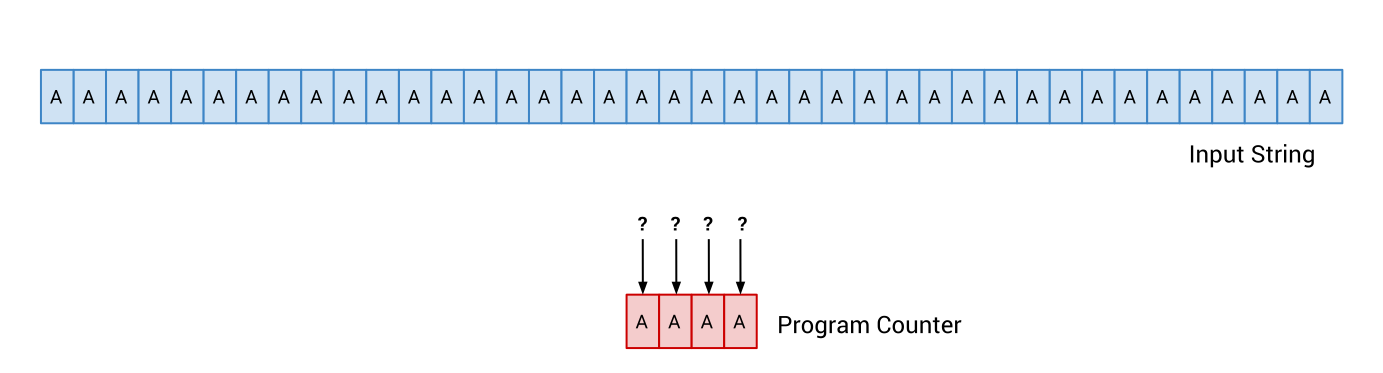
\includegraphics[width=\textwidth]{blind-program-counter-contamination}
  \caption{Vague relationship between input string and program counter}
  \label{fig:blind-program-counter-contamination}
\end{figure}

\begin{figure}[!ht]
  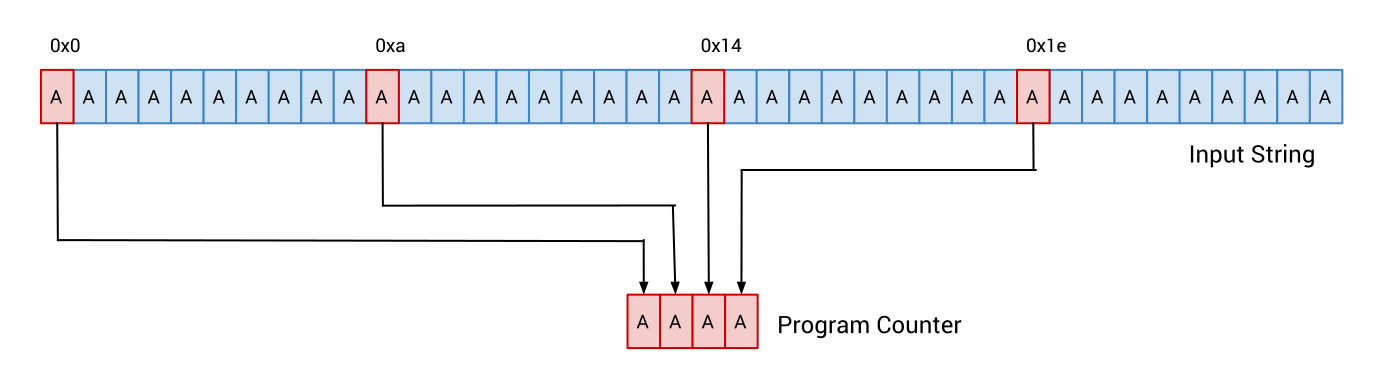
\includegraphics[width=\textwidth]{program-counter-contamination}
  \caption{Clear relationship between input string and program counter}
  \label{fig:program-counter-contamination}
\end{figure}

\emph{CRAX} makes this process easy relying on symbolic execution. A hacker
first symbolizes the input string, the input string thereby becomes expressions
instead of constant values. For example, reading from the first byte of the
string results in the expression ``(ReadLSB w8 0x0 v0\_symdata\_0)'' instead of
the original value `A'. The expression means ``Reads 8 bits starting from
offset 0 of symbolic value v0\_symdata\_0''. When PC is found tainted, with the
example we just mentioned, instead of ``AAAA'', an expression like
Listing~\ref{lst:concat-expression} will be retrieved. The result clearly shows
that PC is overwritten by a string concatenated by offset 0x0 (1st),
0xa (11th), 0x14 (21st), and 0x1e (31st) of v0\_symdata\_0, as shown in
Figure~\ref{fig:program-counter-contamination}.

\begin{listing}[H]
  \begin{minted}{text}
  (Concat w32 (ReadLSB w8 0x1e v0_symdata_0)
              (Concat w24 (ReadLSB w8 0x14 v0_symdata_0)
                          (Concat w16 (ReadLSB w8 0xa v0_symdata_0)
                                      (ReadLSB w8 0x0 v0_symdata_0))))
  \end{minted}
  \caption{Expression of concatenating 1st, 11th, 21st and 31st bytes}
  \label{lst:concat-expression}
\end{listing}

\begin{figure}[!ht]
  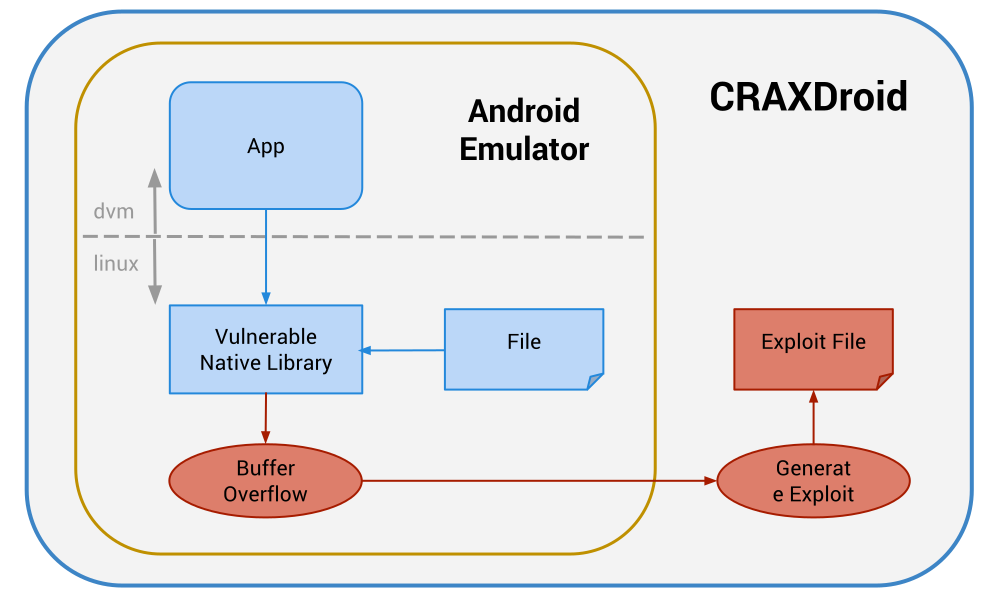
\includegraphics[width=\textwidth]{android-exploit-scenario}
  \caption{An Exploit Scenario on Android}
  \label{fig:android-exploit-scenario}
\end{figure}

To further generate exploit for a vulnerable shared library of a Android app, a
scenario is presented as Figure~\ref{fig:android-exploit-scenario} shown.
Suppose a app uses a shared library, which reads from local files and then copy
the content into local buffers using dangerous functions, for example,
\textbf{strcpy} or \textbf{strncpy}. The first step is to feed a file that will
trigger the vulnerability. \emph{CRAX} installs a sensor at the place where the
PC register updates value. Once the sensor detects that the value contains
symbolic expressions instead of constant value, the exploit generating process
starts.

\begin{figure}[!ht]
  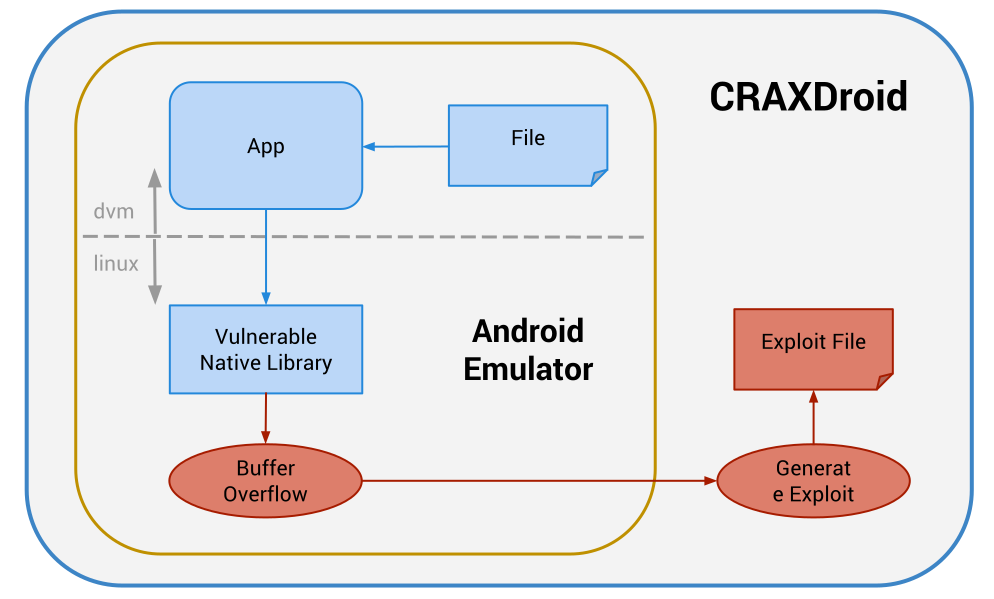
\includegraphics[width=\textwidth]{android-exploit-scenario2}
  \caption{Another Exploit Scenario on Android}
  \label{fig:android-exploit-scenario2}
\end{figure}

The previous scenario takes place underneath Dalvik VM completely, which makes
it almost no different from exploiting an ordinary linux application. To let
\emph{CRAXDroid} better live up to its name, another scenario is designed. As
shown in Figure~\ref{fig:android-exploit-scenario2}, this scenario is almost
identical to the previous one, except the input file is read by the Dalvik VM
instead of the shared library. Although a small change, it makes big different.

Symbolic execution lives on symbol propagating and constraints collecting. When
execution comes to a conditional branch, for example, \textbf{jz},
\textbf{jnz}, \textbf{jge}, etc., and a operand is symbolized, the execution
engine will collect the constraint, named ``path constraint''. The path
constraints that would eventually lead to the ``success'' in
Listing~\ref{lst:simple-branching} would be resolved to
Listing~\ref{lst:simple-branching-constraints}. Given a solver the path
constraint, it will generate solutions that satisfy the constraint, such as the
string ``Y\textless A''.

\begin{listing}[H]
  \begin{minted}[linenos]{c}
  if (data[0] != 'Z') {
      if (data[1] != '>') {
          if (data[2] != 'B') {
              print('success');
          }
      }
  }
  \end{minted}
  \caption{An Example of Simple Branching}
  \label{lst:simple-branching}
\end{listing}

\begin{listing}[H]
  \begin{minted}{text}
  (And w8 (Eq false
              (Eq (w8 0x42)
                  (ReadLSB w8 0x2 v0_symdata_0)))
          (And w8 (Eq false
                      (Eq (w8 0x31)
                          (ReadLSB w8 0x1 v0_symdata_0)))
                  (Eq false
                      (Eq (w8 0x5a)
                          (ReadLSB w8 0x0 v0_symdata_0)))))
  \end{minted}
  \caption{The path constraint generated from Listing~\ref{lst:simple-branching}}
  \label{lst:simple-branching-constraints}
\end{listing}

Back to the scenario, since we don't know whether symbol propagating would work
properly inside Dalvik VM, the first scenario is designed as a quick proof of
concept to prove that there are chances that vulnerabilities would hide under
shared libraries and \emph{CRAXDroid} is capable of exploiting them. The second
scenario intends to prove that symbols would be propagated through Dalvik VM
and contaminate shared libraries without problems. Therefore, not only files,
more sources would start to become dangerous.
